\section{Validación y resultados}
\label{sec:results}

\subsection{Resultados de preparación de datos}

La preparación del dataset permitió pasar de un export con fuga entre splits a un
conjunto trazable. Los principales resultados de esta etapa son:

\begin{itemize}
  \item 4.212 archivos originales analizados; 1.754 clusters/originales identificados.
  \item 55 descartes por duplicados o casi-duplicados en evaluación.
  \item 284 pares de casi-duplicados entre clusters y 22 conflictos de etiqueta
        documentados.
  \item Split limpio sin intersección de clusters: 3.428 train, 209 valid, 146 test.
  \item Versión limpia para entrenamiento: 1.325 train, 209 valid, 146 test, con una
        imagen por cluster y exclusión de conflictos de etiqueta.
\end{itemize}

La limpieza de conflictos es relevante porque varias confusiones esperadas ocurren
entre clases visualmente similares, en especial \emph{chert}, \emph{diatomite} y
\emph{siliceous-sinter} (geiserita). La Figura~\ref{fig:siliceas} ilustra ejemplos
de procesos asociados a estas clases.

\begin{figure}[H]
  \centering
  \begin{minipage}{0.48\linewidth}
    \centering
    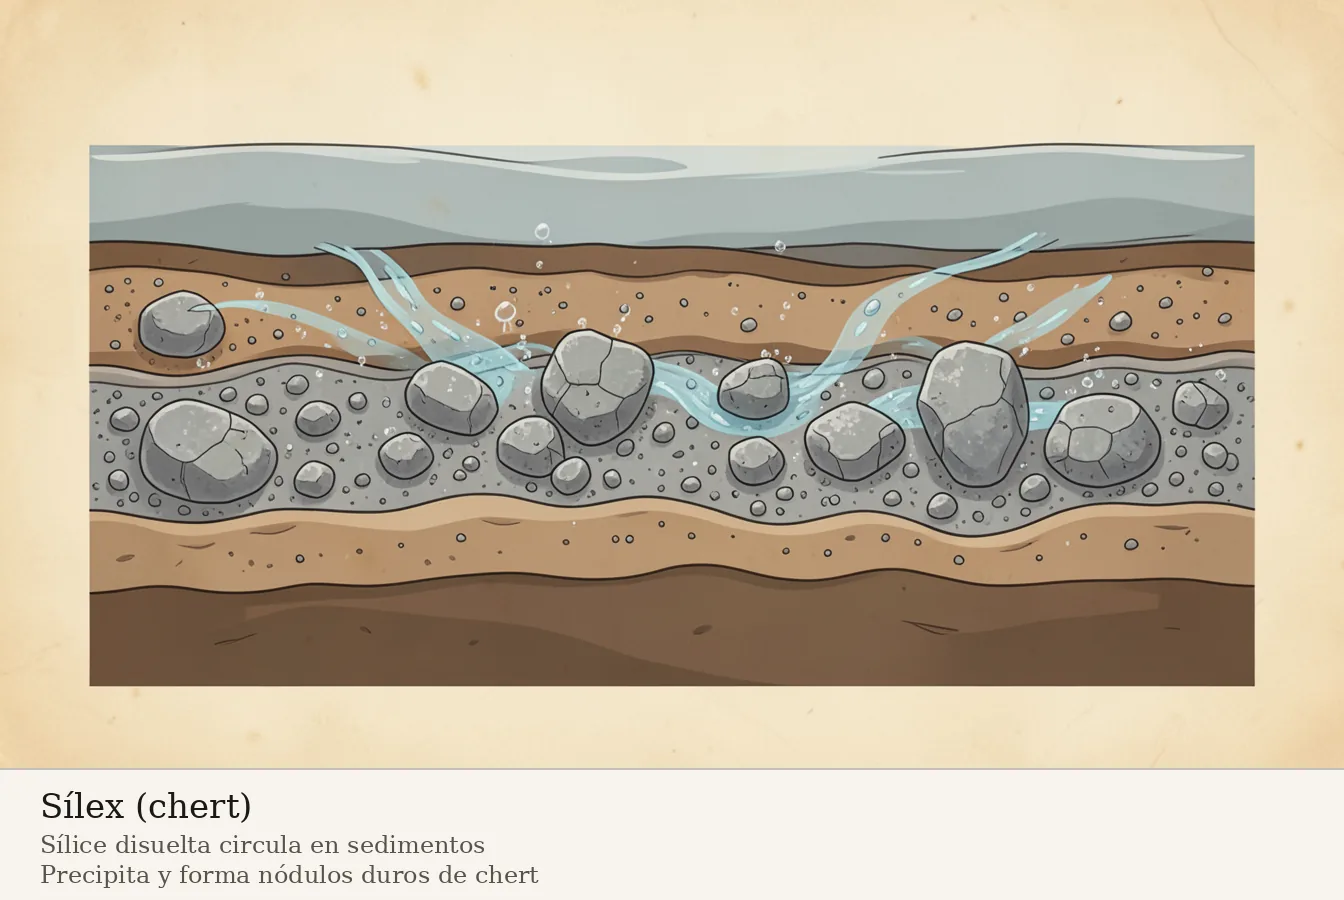
\includegraphics[width=\linewidth]{assets/images/chert.png}
  \end{minipage}\hfill
  \begin{minipage}{0.48\linewidth}
    \centering
    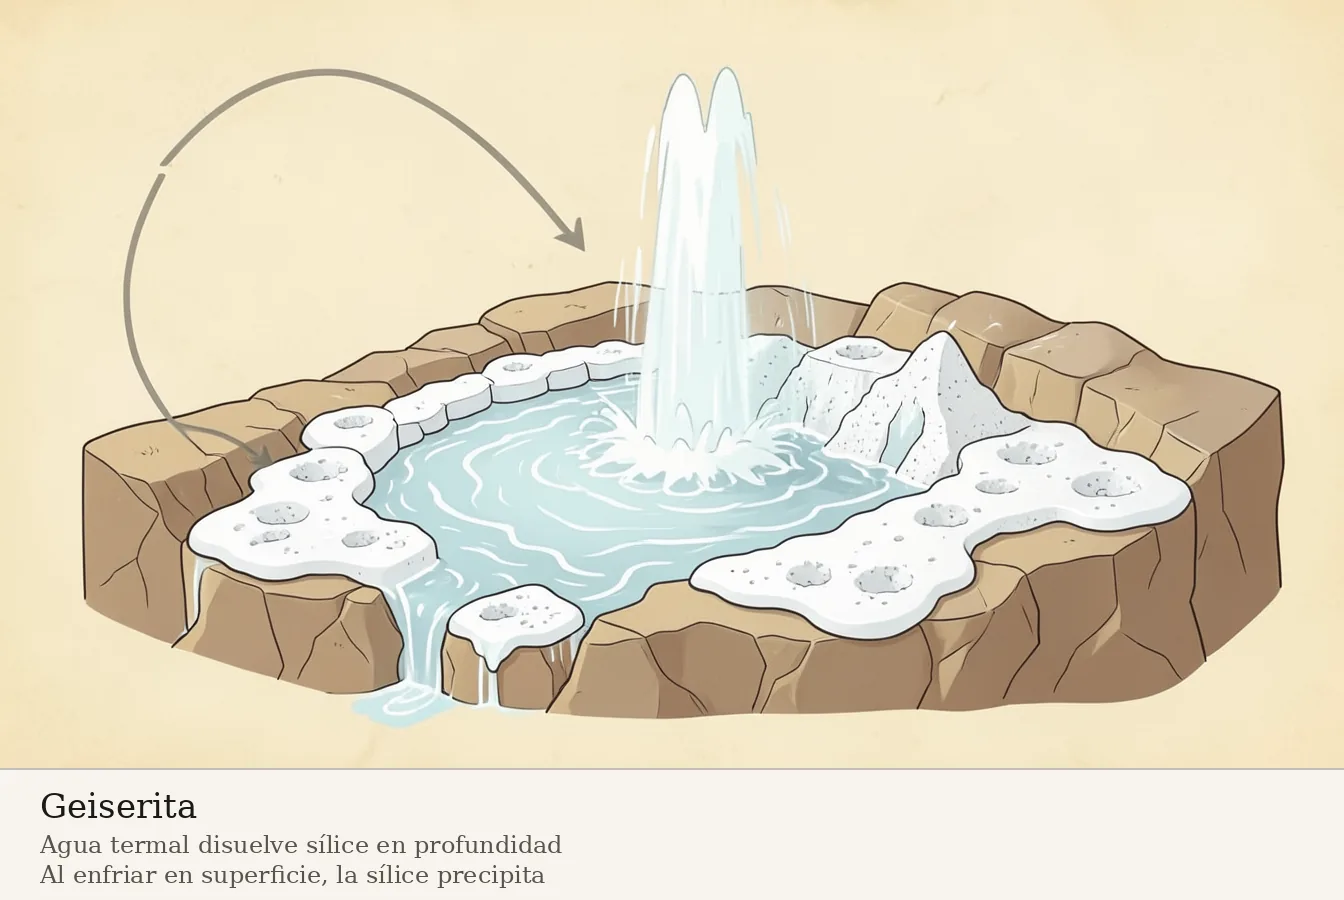
\includegraphics[width=\linewidth]{assets/images/siliceous-sinter.png}
  \end{minipage}
  \caption{Ejemplos de ilustraciones de proceso para clases síliceas}
  \label{fig:siliceas}
\end{figure}

\subsection{Estado de la aplicación}

La aplicación Litoteca se encuentra desplegada en Cloudflare Pages
\cite{litotecaapp}. El repositorio público está en GitHub \cite{litotecarepo}. La
Tabla~\ref{tab:funcionalidades} resume el estado de las funcionalidades relevantes
para la entrega.

\begin{table}[H]
  \centering
  \caption{Estado de funcionalidades implementadas}
  \label{tab:funcionalidades}
  \begin{tabular}{@{}p{4.3cm}p{8.1cm}@{}}
    \toprule
    Funcionalidad & Estado \\
    \midrule
    Carga/captura de imagen & Implementada, con validación de tipo y tamaño. \\
    Ficha por clase & Implementada para las 9 clases, con extractos cacheados de Wikipedia~\cite{wikipedia}. \\
    Historial local & Implementado con \texttt{localStorage}. \\
    Proxy de predicción & Implementado en \texttt{functions/api/predict.js}. \\
    Guardrail roca/no-roca & Implementado; el detector binario se consulta antes del clasificador y responde HTTP 422 con código \texttt{no\_es\_roca}. \\
    Modo sin conexión & Implementado con service worker y mensaje honesto para predicción en línea~\cite{w3cserviceworkers}. \\
    Despliegue CF Pages & Implementado con GitHub Actions y Wrangler. \\
    Modelo Advanced & Publicado como \texttt{litoteca-v2} y conectado como clasificador final (P 98.66\%, R 96.22\%, AP 98.42\%). \\
    Quick v3 evaluado & Completado (P 79.70\%, R 54.58\%, AP 74.64\%; validación API 96/146, 65.75\%); no superó a Quick v2, no se promovió. \\
    \bottomrule
  \end{tabular}
\end{table}

\begin{figure}[H]
  \centering
  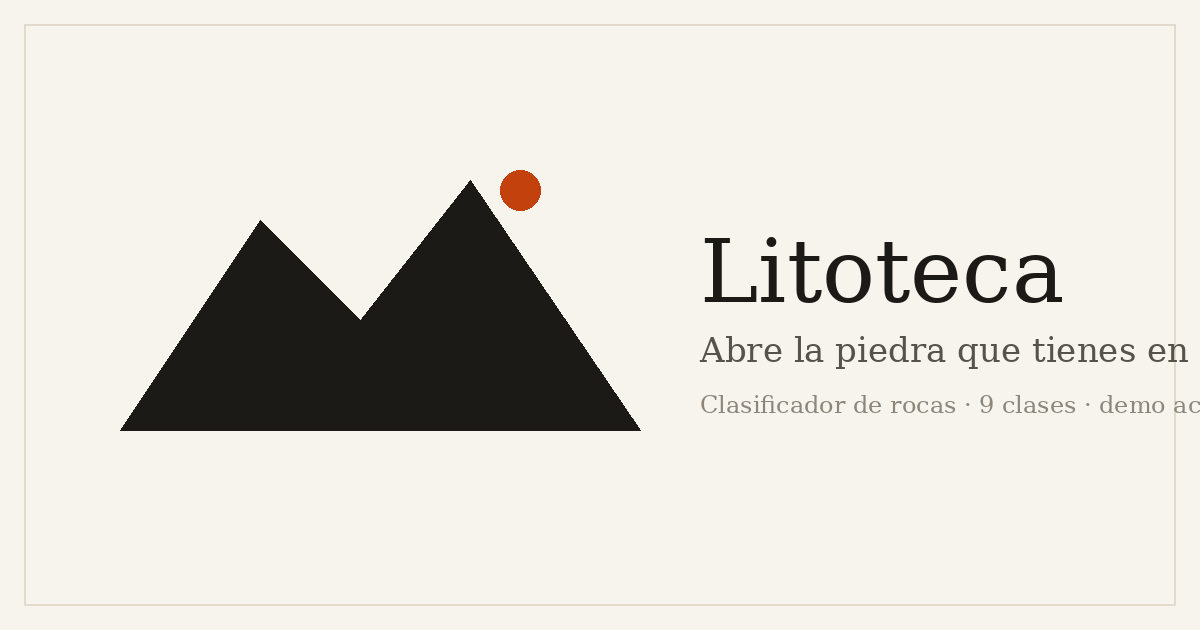
\includegraphics[width=0.75\linewidth]{assets/images/og-image.png}
  \caption{Vista de identidad visual de Litoteca}
  \label{fig:og}
\end{figure}

\subsection{Validación sintética por API}

Se ejecutó una validación sintética contra la iteración publicada actualmente como
\texttt{litoteca-v2} (Advanced, \texttt{d538f641-63da-4db3-8827-fe2e1f91cee9}) usando
el conjunto \texttt{data/prepared-clean-train/test} (146 imágenes, una por cluster,
sin fuga). La llamada se realizó al endpoint de predicción de Custom Vision con el
mismo contrato que consume la aplicación.

\begin{table}[H]
  \centering
  \caption{Validación sintética por API (test limpio, Advanced)}
  \label{tab:api-test}
  \begin{tabular}{@{}lrrr@{}}
    \toprule
    Clase & Aciertos & Total & Accuracy \\
    \midrule
    basalt & 14 & 15 & 93.33\% \\
    chert & 11 & 14 & 78.57\% \\
    clay & 6 & 12 & 50.00\% \\
    conglomerate & 9 & 13 & 69.23\% \\
    diatomite & 12 & 19 & 63.16\% \\
    gypsum & 19 & 23 & 82.61\% \\
    olivine-basalt & 18 & 19 & 94.74\% \\
    shale & 11 & 20 & 55.00\% \\
    siliceous-sinter & 9 & 11 & 81.82\% \\
    \midrule
    \textbf{Total} & \textbf{109} & \textbf{146} & \textbf{74.66\%} \\
    \bottomrule
  \end{tabular}
\end{table}

Frente a Quick v2 (101/146, 69.18\%), la iteración Advanced mejora en 8 aciertos
(+5.48 puntos porcentuales). Los errores remanentes se concentran en clases
visualmente cercanas: \emph{conglomerate}$\rightarrow$\emph{siliceous-sinter} (3),
\emph{diatomite}$\rightarrow$\emph{chert} (3),
\emph{shale}$\rightarrow$\emph{conglomerate} (3),
\emph{chert}$\rightarrow$\emph{diatomite} (2),
\emph{clay}$\rightarrow$\emph{shale} (2),
\emph{clay}$\rightarrow$\emph{siliceous-sinter} (2),
\emph{shale}$\rightarrow$\emph{chert} (2),
\emph{shale}$\rightarrow$\emph{diatomite} (2) y
\emph{siliceous-sinter}$\rightarrow$\emph{chert} (2). La mejora es consistente con
las métricas de entrenamiento y reduce la brecha entre validación y uso real.
